% Provenance (never printed): see sources/outline_sources.md (Year 2: climate archives and proxies;
% foraminiferal and ice isotopes; Mg/Ca; pollen; speleothems; tree rings; dating the archives).
% Calibrations after Miller et al. (2020), Groeneveld et al. (2019) and Morley et al. (2024); ice
% cores after White (Geochemistry, ch. 9), Werner et al. (2018) and the EPICA Dome C file of Jouzel
% et al. (2007); age model after Svensson et al. (2008); deep-water context after Wharton et al.
% (2026); figures from figdata/bachelor-2/proxies.py (data/derived lr04, edc-temperature,
% co2-icecore); values of the exercises and problem computed in the Book 4 scratch calculator
% calc/ch24.py.
\chapter{Archivos e indicadores climáticos}\label{ch:b2:climate-proxies}

En un artículo de 1955, un joven geoquímico dio a conocer los isótopos del oxígeno de los diminutos caparazones de
foraminíferos extraídos de testigos del fondo oceánico, y encontró en ellos quince ciclos glaciares--interglaciares en los
últimos \num{600000} años. Los leyó sobre todo como temperatura: atribuyó solo una quinta parte, aproximadamente, de
las oscilaciones al hielo almacenado en tierra. Dieciocho años después, Shackleton y Opdyke concluyeron lo
contrario: el efecto principal era el almacenamiento de agua isotópicamente ligera en los casquetes
de hielo. Los mismos caparazones, las mismas cifras, dos lecturas. Un caparazón de calcita registra la
temperatura del agua en la que creció y la composición de esa agua, y la composición del
agua de mar depende de cuánto hielo hay en tierra. Este capítulo trata de esos registros, de los
archivos que los conservan, de los indicadores que se leen en ellos, de cómo se calibran frente a los termómetros
y de cómo se datan, y del arte de separar dos señales transportadas por un mismo caparazón.
% ledger: white13c9:paleo-history

\begin{recall}
\textbf{De los volúmenes escolares}: \omterm{def:b2:climate-proxies:proxy}{archivo climático} e indicador indirecto, testigo de hielo, periodo glaciar e
interglaciar, el Último Máximo Glacial (hace unos \num{23000} a \num{19000} años), el análisis
polínico. \textbf{Del volumen de primer año}: la datación radiométrica, la edad radiocarbono y su
curva de calibración; el fango calcáreo, formado por cocolitos y caparazones de foraminíferos.
\textbf{Del \cref{ch:b2:isotope-geochemistry}}: los patrones isotópicos de referencia \omterm{def:b2:isotope-geochemistry:standards}{VSMOW} y \omterm{def:b2:isotope-geochemistry:standards}{VPDB}
(\cref{def:b2:isotope-geochemistry:standards}) y la \omterm{prop:b2:isotope-geochemistry:mwl}{recta de agua meteórica}, $\delta\mathrm{D}
\approx 8\,\delta^{18}\mathrm{O} + 10$ (\cref{prop:b2:isotope-geochemistry:mwl}). \textbf{De los
libros de química}: el valor $\delta$ y el factor de fraccionamiento. \textbf{De los libros de
matemáticas}: la recta de mínimos cuadrados.
\end{recall}
% ledger: ipcc:lgm-cooling, kc98:mwl, kc98:standards

\section{Archivos e indicadores}\label{sec:b2:climate-proxies:archives}

Los instrumentos solo miden el clima desde hace poco. Todo lo anterior se lee en materiales
que crecieron o se depositaron capa a capa mientras el clima actuaba sobre ellos: la nieve que se convierte en hielo en los
casquetes polares, los caparazones que llueven sobre el fondo oceánico, los anillos de los árboles, los corales, los depósitos de
las cuevas, el fango de los lagos. Los volúmenes escolares los llamaban archivos, y a las magnitudes medidas en
ellos, indicadores indirectos; ahora necesitamos palabras más precisas.

\begin{definition}[Archivo climático; indicador climático indirecto]\label{def:b2:climate-proxies:proxy}
Un \emph{archivo climático}\index{archivo climatico@archivo climático} es un material natural que se acumula
progresivamente, capa sobre capa o anillo sobre anillo, y conserva características físicas, químicas o biológicas
del ambiente en el que se formó cada parte. Un \emph{indicador climático
indirecto}\index{indicador climatico indirecto@indicador climático indirecto} es una magnitud medida en un archivo que depende de una variable
climática, como una temperatura, una cantidad de lluvia o un volumen de hielo, a través de una relación que puede
calibrarse, y que sustituye así a una medida de esa variable que nunca se hizo.
\end{definition}
% ledger: ncei:proxy, ncei:paleocean

Tres propiedades deciden lo que puede contar un archivo: su resolución (el intervalo de tiempo cubierto por una
muestra), su alcance (hasta dónde se remonta) y cómo se data. Un archivo con capas anuales puede
leerse año a año y datarse contando; los demás necesitan edades radiométricas o la comparación con un
registro datado. La tabla de abajo compara los archivos de este capítulo.

\begin{center}
\small
\begin{tabular}{>{\raggedright\arraybackslash}p{0.17\linewidth}>{\raggedright\arraybackslash}p{0.27\linewidth}>{\raggedright\arraybackslash}p{0.21\linewidth}>{\raggedright\arraybackslash}p{0.24\linewidth}}
\hline
archivo & indicadores en este capítulo & capas anuales & datación \\
\hline
sedimento de mar profundo & $\delta^{18}$O y Mg/Ca de foraminíferos & no & radiocarbono, comparación con
registros datados \\
hielo polar & $\delta$D y $\delta^{18}$O del hielo, aire de las burbujas & en la parte superior de los testigos
gruesos & recuento de capas, capas volcánicas datadas \\
anillos de los árboles & anchura de los anillos, densidad de la madera, isótopos & sí & recuento y \omterm{def:b2:climate-proxies:dendro}{sincronización} de anillos \\
\omterm{def:b2:climate-proxies:archives}{espeleotemas} & $\delta^{18}$O & en algunos & datación radiométrica \\
sedimentos lacustres & \omterm{def:b2:climate-proxies:archives}{varvas}, polen & donde hay \omterm{def:b2:climate-proxies:archives}{varvas} & recuento de \omterm{def:b2:climate-proxies:archives}{varvas} \\
\hline
\end{tabular}
\end{center}
% ledger: ncei:proxy, ncei:paleocean, ncei:tree-ring, ncei:speleothem, mccarthy23:varves, svensson08:gicc05, noaa:gisp2-layers, bebchuk26:crossdating

Un indicador nunca es una medida pura de una sola variable. La anchura de un anillo de árbol depende del calor
del verano y de la lluvia; el $\delta^{18}$O de un caparazón, de la temperatura del agua y de
su composición isotópica. El trabajo del paleoclimatólogo consiste en encontrar un indicador cuya dependencia
de la variable buscada sea fuerte y conocida, medir las demás influencias de forma independiente y
datar la muestra.

\section{Los isótopos del oxígeno en los caparazones carbonatados}\label{sec:b2:climate-proxies:oxygen}

Los foraminíferos son protistas unicelulares, muchos de los cuales construyen un caparazón de calcita; las especies
planctónicas flotan en las aguas superficiales, las bentónicas viven sobre el sedimento del fondo marino o dentro de él.
Sus caparazones se acumulan en los fangos calcáreos del volumen de primer año, y el
$\delta^{18}$O de la calcita puede medirse en unos pocos caparazones extraídos de cada centímetro de un
testigo.
% ledger: ucmp:forams, ncei:paleocean

\begin{history}[Dos lecturas de un mismo registro]
Urey calculó en 1947 cómo depende de la temperatura el fraccionamiento del oxígeno entre la calcita y el agua,
y propuso que los carbonatos podían registrar la temperatura a la que se formaron. Cesare
Emiliani, entonces su alumno, midió el $\delta^{18}$O de foraminíferos de testigos de pistón de los
océanos del mundo y publicó en 1955 un registro con 15 ciclos glaciares--interglaciares en
\num{600000} años, atribuyendo alrededor del \qty{20}{\percent} de la variación al volumen de hielo.
En 1973 Shackleton y Opdyke concluyeron que el almacenamiento de agua isotópicamente ligera en los
casquetes de hielo era el efecto principal. Los efectos vitales, las desviaciones de una especie respecto del equilibrio,
y el intercambio de oxígeno con el agua intersticial tras el enterramiento no suelen tener mucha importancia para los
caparazones de los últimos millones de años; la composición isotópica del agua sí la tiene.
\end{history}
% ledger: white13c9:paleo-history

\subsection*{La temperatura}

La calcita que crece en equilibrio con el agua es más rica en \textsuperscript{18}O que el agua,
y cuanto más fría el agua, mayor el enriquecimiento, como mostró el cálculo de Urey. Varias
calibraciones empíricas relacionan
la temperatura con la diferencia entre el $\delta^{18}$O de la calcita, en la escala \omterm{def:b2:isotope-geochemistry:standards}{VPDB}, y
el del agua, en la escala \omterm{def:b2:isotope-geochemistry:standards}{VSMOW}. Para el mar profundo se usa una forma simplificada para los caparazones
bentónicos.

\begin{proposition}[Una calibración bentónica]\label{prop:b2:climate-proxies:benthic}
Para los foraminíferos bentónicos a temperaturas de mar profundo (por debajo de unos \qty{13}{\celsius}),
\[
  T = 16.1 - 4.76\,\bigl[\delta^{18}\mathrm{O}_{\mathrm{b}} - (\delta^{18}\mathrm{O}_{\mathrm{sw}} -
  0.27)\bigr],
\]
con $T$ en \unit{\celsius}, $\delta^{18}\mathrm{O}_{\mathrm{b}}$ el valor del caparazón (por mil,
\omterm{def:b2:isotope-geochemistry:standards}{VPDB}) y $\delta^{18}\mathrm{O}_{\mathrm{sw}}$ el del agua de mar (por mil, \omterm{def:b2:isotope-geochemistry:standards}{VSMOW}); el término
0.27 pasa el agua a la escala de la calcita. Un enfriamiento de \qty{1}{\celsius} con composición del agua
constante aumenta $\delta^{18}\mathrm{O}_{\mathrm{b}}$ en $1/4.76 = 0.21$ por mil.
\end{proposition}
\admitted
% ledger: miller20:paleotemp, groeneveld19:anand

La ecuación más completa de la que se simplifica lleva un pequeño término cuadrático,
$T = 16.1 - 4.64x + 0.09x^2$ con $x$ la diferencia de los dos valores $\delta$; los caparazones planctónicos
tienen sus propias calibraciones, de la misma forma, como $T = 14.9 - 4.8\,[\delta^{18}\mathrm{O} -
(\delta^{18}\mathrm{O}_{\mathrm{sw}} - 0.27)]$. Todas comparten una dificultad: el caparazón da un
número, $\delta^{18}\mathrm{O}_{\mathrm{b}}$, y la ecuación tiene dos incógnitas, $T$ y
$\delta^{18}\mathrm{O}_{\mathrm{sw}}$. Hace falta un segundo indicador, independiente, para separarlas.
% ledger: miller20:paleotemp, groeneveld19:anand

\subsection*{El efecto del volumen de hielo}

El agua que se evapora del mar lleva menos \textsuperscript{18}O que el mar; a medida que el vapor
viaja hacia el polo y precipita en forma de lluvia o nieve, se empobrece aún más, y la nieve que forma los casquetes
de hielo es una de las aguas más ligeras del planeta: el hielo de Groenlandia tiene un $\delta^{18}$O de $-30$ a $-35$
por mil, el de la Antártida baja hasta $-50$. Cuando los casquetes crecen, el isótopo ligero queda retenido en tierra
y el océano que queda se vuelve más pesado.
% ledger: nasaeo:o18, white:d18o

\begin{definition}[Efecto del volumen de hielo]\label{def:b2:climate-proxies:ice-volume}
El \emph{efecto del volumen de hielo}\index{efecto del volumen de hielo} es el cambio de la composición
isotópica del oxígeno de todo el océano causado por el crecimiento o el retroceso de los casquetes de hielo continentales, que
almacenan agua empobrecida en \textsuperscript{18}O; desplaza el $\delta^{18}$O de todo carbonato
formado en el mar en la misma cantidad, cualquiera que sea la temperatura.
\end{definition}
% ledger: nasaeo:o18, white13c9:ice-volume, miller20:paleotemp

\begin{omfigure}
\centering
\begin{tikzpicture}[font=\scriptsize, >=Stealth]
\foreach \col/\title in {0/{a\enspace hoy}, 7.0/{b\enspace un máximo glaciar}} {
  \begin{scope}[shift={(\col,0)}]
  \node[anchor=south west] at (0,3.3) {\textbf{\title}};
  \fill[brown!30] (3.6,0) -- (6.4,0) -- (6.4,1.6) -- (3.6,1.2) -- cycle;
  \end{scope}
}
% today: full ocean, small ice sheet
\fill[ocBlue!25] (0,0) rectangle (3.6,1.2);
\node[align=center] at (1.75,0.55) {océano\\$\delta^{18}\mathrm{O} = 0$};
\fill[white, draw=black!50] (5.2,1.43) .. controls (5.6,1.95) and (6.2,1.95) .. (6.4,1.6) -- cycle;
\node at (5.0,0.65) {hielo, $-40$};
\draw[black!50] (5.0,0.85) -- (5.7,1.55);
\draw[->, thick, ocBlue] (1.6,1.35) .. controls (2.4,2.9) and (4.6,2.9) .. (5.6,2.05);
\node at (3.4,3.0) {vapor, ligero};
% glacial: lower sea, big ice sheet
\begin{scope}[shift={(7.0,0)}]
\fill[ocBlue!35] (0,0) rectangle (3.6,0.85);
\draw[densely dashed] (0,1.2) -- (3.6,1.2);
\node[anchor=south west, align=left] at (0.05,1.2) {nivel del mar\\actual};
\draw[<->] (3.35,0.85) -- (3.35,1.2);
\node[anchor=east] at (3.3,1.02) {\qty{130}{m}};
\node[align=center] at (1.6,0.42) {océano, $\delta^{18}\mathrm{O} = +1.46$};
\fill[white, draw=black!50] (3.6,1.2) .. controls (4.0,2.6) and (6.0,2.7) .. (6.4,1.6) -- cycle;
\node at (5.1,1.85) {hielo, $-40$};
\draw[->, thick, ocBlue] (2.15,0.9) .. controls (2.3,2.6) and (3.3,3.0) .. (4.3,2.6);
\end{scope}
\end{tikzpicture}
\par\smallskip{\small El \omterm{def:b2:climate-proxies:ice-volume}{efecto del volumen de hielo} (esquema, sin escala): el vapor que alimenta los casquetes
de hielo está empobrecido en \textsuperscript{18}O, así que almacenar \qty{130}{m} de nivel del mar en forma de hielo de
$\delta^{18}\mathrm{O} = -40$ por mil deja el océano \num{1.46} por mil más pesado
(\cref{prop:b2:climate-proxies:mass-balance}). Valores en por mil, \omterm{def:b2:isotope-geochemistry:standards}{VSMOW}.}
\end{omfigure}
% ledger: nasaeo:o18, miller20:ice-cal, ipcc:lgm-sea

¿De qué tamaño es el desplazamiento? Lo da un balance de masas, si se conocen el volumen del hielo y su composición
isotópica media.

\begin{proposition}[Efecto del volumen de hielo por balance de masas]\label{prop:b2:climate-proxies:mass-balance}
Sea el océano actual de profundidad media $H$ y con un $\delta^{18}$O de 0 (\omterm{def:b2:isotope-geochemistry:standards}{VSMOW}). Si se retira una capa de agua
de mar de espesor $h$ y se almacena en tierra como hielo de composición media
$\delta_{\mathrm{ice}}$, manteniendo fija el área del océano, el océano restante tiene
\[
  \Delta\delta^{18}\mathrm{O}_{\mathrm{sw}} = \frac{-h\,\delta_{\mathrm{ice}}}{H - h}.
\]
Para $h$ pequeño, el desplazamiento crece de forma casi lineal, en $-\delta_{\mathrm{ice}}/H$ por metro de nivel del mar.
\end{proposition}

\begin{proof}
Para un isótopo minoritario, los valores $\delta$ se combinan como concentraciones: el $\delta$ de una mezcla es
la media de los valores $\delta$ de sus partes ponderada por sus cantidades de oxígeno, y todas las
partes son aquí agua. Por unidad de área oceánica, el agua del océano actual, una columna $H$ con
$\delta = 0$, se reparte entre el hielo, $h$ con $\delta_{\mathrm{ice}}$, y el océano restante,
$H - h$ con $\Delta\delta^{18}\mathrm{O}_{\mathrm{sw}}$:
$H \times 0 = h\,\delta_{\mathrm{ice}} + (H - h)\,\Delta\delta^{18}\mathrm{O}_{\mathrm{sw}}$, lo que
da la fórmula. Para $h \ll H$, $H - h \approx H$.
\end{proof}
% ledger: white13c9:ice-mass, charette:ocean-volume

\begin{example}[El océano del último máximo glaciar]\label{ex:b2:climate-proxies:lgm}
En el Último Máximo Glacial el nivel del mar estaba de 125 a \qty{134}{m} por debajo del actual; tómense \qty{130}{m},
con $H = \qty{3682.2}{m}$, y hielo a $-40$ por mil, el valor inferido para el gran casquete de
América del Norte. Entonces
$\Delta\delta^{18}\mathrm{O}_{\mathrm{sw}} = 130 \times 40/(3682.2 - 130) = 5200/3552.2 = 1.46$
por mil, unos $40/3682.2 = 0.0109$ por mil por metro de nivel del mar. Las comparaciones con curvas del nivel del mar
obtenidas de terrazas y arrecifes de coral datados dan \num{0.011} por mil por metro, de acuerdo con ello; una escala de
\num{0.13} por mil por cada \qty{10}{m}, usada en algunas reconstrucciones, corresponde a hielo a unos
$-50$ por mil. Una medida directa del cambio, a partir del $\delta^{18}$O del agua que aún retienen
los poros del sedimento glaciar, da $1.0 \pm 0.1$ por mil.
\end{example}
% ledger: ipcc:lgm-sea, charette:ocean-volume, miller20:ice-cal, white13c9:ice-volume, wharton26:deep

La figura de abajo muestra cuánto depende la respuesta de la composición supuesta para el hielo.
La diferencia entre \num{1.0} y \num{1.5} por mil no es pequeña: a \num{0.21} por mil por grado,
equivale a más de dos grados de temperatura del océano profundo. La relación tampoco es del todo
lineal: el océano que queda se reduce a medida que crece el hielo, y el $\delta^{18}$O medio del propio hielo
cambia a medida que crecen y retroceden casquetes de composición distinta. Por eso las reconstrucciones del nivel del mar
a partir del $\delta^{18}$O suelen usar una relación lineal calibrada con el valor del agua intersticial, aun
reconociendo que la relación verdadera debería ser no lineal.
% ledger: wharton26:deep, rohling21:linear, miller20:paleotemp

\begin{omfigure}
\centering
% figdata/bachelor-2/proxies.py part icevol
\begin{tikzpicture}
\begin{axis}[width=0.86\linewidth, height=6.0cm, xmin=0, xmax=150, ymin=0, ymax=2.2,
  xlabel={agua de mar almacenada como hielo, $h$ (\unit{m} de nivel del mar)},
  ylabel={$\Delta\delta^{18}\mathrm{O}_{\mathrm{sw}}$ (por mil)},
  tick label style={font=\scriptsize}, label style={font=\small}, xtick={0,25,...,150},
  legend style={font=\scriptsize, at={(0.5,1.02)}, anchor=south, draw=none, legend columns=4,
  /tikz/every even column/.append style={column sep=6pt}}, legend cell align=left]
\fill[black!10] (axis cs:125,0) rectangle (axis cs:134,2.2);
\addplot[ocBlue, thick] table[x=h_m, y=d30] {figdata/out/bachelor-2-proxies-icevol.dat};
\addlegendentry{hielo a $-30$}
\addplot[black, thick] table[x=h_m, y=d40] {figdata/out/bachelor-2-proxies-icevol.dat};
\addlegendentry{hielo a $-40$}
\addplot[ocRed, thick] table[x=h_m, y=d50] {figdata/out/bachelor-2-proxies-icevol.dat};
\addlegendentry{hielo a $-50$}
\addplot[only marks, mark=square*, mark size=1.8pt, omDef, error bars/.cd, y dir=both,
  y explicit] coordinates {(130,1.0) +- (0,0.1)};
\addlegendentry{agua intersticial}
\addplot[black!60, densely dashed, domain=0:150, samples=2, forget plot] {1.69};
\node[font=\scriptsize, anchor=south west] at (axis cs:3,1.69) {cambio total de LR04, 1.69};
\node[font=\scriptsize, anchor=north, align=center] at (axis cs:112,0.45) {último máximo\\glaciar
$\rightarrow$};
\end{axis}
\end{tikzpicture}
\par\smallskip{\small El \omterm{def:b2:climate-proxies:ice-volume}{efecto del volumen de hielo} según el balance de masas de la
\cref{prop:b2:climate-proxies:mass-balance}, para tres composiciones del hielo (por mil, \omterm{def:b2:isotope-geochemistry:standards}{VSMOW});
banda gris: el descenso del nivel del mar del Último Máximo Glacial, de 125 a \qty{134}{m}; cuadrado: el cambio
medido en las aguas intersticiales de los sedimentos, $1.0 \pm 0.1$ por mil, situado en \qty{130}{m}; en trazos: el
cambio del registro apilado bentónico entre hoy y el Último Máximo Glacial.}
\end{omfigure}
% ledger: ipcc:lgm-sea, wharton26:deep, data:b4-proxies, miller20:ice-cal

\subsection*{El registro apilado bentónico}

Los registros del $\delta^{18}$O bentónico de muchos testigos, alineados y promediados, forman un registro apilado cuyo ruido
es menor que el de cualquier testigo aislado. El registro apilado LR04 combina 57 registros de sitios repartidos por
el océano mundial y abarca 5.3 millones de años. Entre hoy, \num{3.23} por mil, y la media de
\num{19} a \qty{23}{ka}, \num{4.92} por mil, cambia en \num{1.69} por mil, más que cualquier
\omterm{def:b2:climate-proxies:ice-volume}{efecto del volumen de hielo} plausible. Como concluyeron Shackleton y Opdyke, la mayor parte del cambio es el hielo;
pero quedan unas décimas de por mil que atribuir al enfriamiento del agua profunda. El problema de este capítulo mide ese residuo.
% ledger: lr04:stack, data:b4-proxies, white13c9:paleo-history, wharton26:deep

\begin{omfigure}
\centering
% figdata/bachelor-2/proxies.py parts lr04, edc, co2
\begin{tikzpicture}
\begin{groupplot}[group style={group size=1 by 3, vertical sep=0.35cm, xlabels at=edge bottom,
  xticklabels at=edge bottom},
  width=0.96\linewidth, height=3.7cm, xmin=0, xmax=800, xtick={0,100,...,800},
  tick label style={font=\scriptsize}, label style={font=\small}]
\nextgroupplot[ylabel={$\delta^{18}\mathrm{O}_{\mathrm{b}}$}, y dir=reverse, ymin=2.45, ymax=5.2,
  ytick={3.5,4.5}]
\addplot[omDef, thin] table[x=age_ka, y=d18O] {figdata/out/bachelor-2-proxies-lr04.dat};
\node[font=\scriptsize, anchor=north east] at (rel axis cs:0.99,0.97) {a\enspace registro apilado LR04 (por
mil, VPDB; eje invertido)};
\nextgroupplot[ylabel={$\Delta T$ (\unit{\celsius})}, ymin=-12, ymax=7, ytick={-10,-5,0,5}]
\addplot[ocBlue, thin] table[x=age_ka, y=dT] {figdata/out/bachelor-2-proxies-edc.dat};
\node[font=\scriptsize, anchor=north east] at (rel axis cs:0.99,0.97) {b\enspace anomalía de temperatura
de EPICA Dome C};
\nextgroupplot[ylabel={CO$_2$ (\unit{ppm})}, ymin=160, ymax=330, ytick={200,250,300},
  xlabel={edad (miles de años antes de 1950)}]
\addplot[ocRed, thin] table[x=age_ka, y=co2] {figdata/out/bachelor-2-proxies-co2.dat};
\node[font=\scriptsize, anchor=north east] at (rel axis cs:0.99,0.97) {c\enspace CO$_2$ del
aire de los testigos de hielo antárticos};
\end{groupplot}
\end{tikzpicture}
\par\smallskip{\small Los últimos \num{800000} años en tres archivos: (a) el registro apilado LR04 del
$\delta^{18}$O bentónico, representado con el eje invertido para que los periodos glaciares apunten hacia abajo; (b) la
anomalía de temperatura en EPICA Dome C, respecto de la media del último milenio, deducida
del $\delta$D del hielo; (c) el CO$_2$ del aire atrapado en el hielo antártico, hasta 1950. Datos: NOAA
NCEI Paleoclimatology (Lisiecki y Raymo 2005; Jouzel et al.\ 2007; Bereiter et al.\ 2015),
descargados el 22 de octubre de 2026.}
\end{omfigure}
% ledger: data:lr04, data:edc-jouzel, data:co2-bereiter, jouzel07:edc-corr, data:b4-proxies

\section{Los testigos de hielo}\label{sec:b2:climate-proxies:ice}

La nieve que cae sobre un casquete de hielo conserva la composición isotópica que tenía al caer, y
cuanto más frío el lugar y la época, más ligera es. En la Antártida, la temperatura media anual del aire y
el $\delta^{18}$O de la nieve siguen una relación lineal estrecha de un sitio a otro, con una
pendiente de unos \num{0.8} por mil por grado, como predice la destilación de Rayleigh del vapor en su camino
hacia el interior. El hidrógeno se usa tanto como el oxígeno: sobre la \omterm{prop:b2:isotope-geochemistry:mwl}{recta de agua meteórica}, $\delta$D varía unas ocho veces más deprisa que $\delta^{18}$O, y
el registro de $\delta$D del hielo antártico se eligió por su mayor sensibilidad a la temperatura.
% ledger: werner18:slopes, white13c9:icecore, kc98:mwl

Una pendiente medida en el espacio no es necesariamente una pendiente en el tiempo. En Groenlandia, donde la
temperatura del propio hielo se ha reconstruido por otros métodos, el cambio de $\delta^{18}$O por grado
a lo largo del tiempo resulta ser de 0.3 a \num{0.6} por mil, frente a una pendiente espacial actual de unos
\num{0.7}: las estaciones de las nevadas, las fuentes de la humedad y sus trayectorias cambiaron con el
clima. Las primeras temperaturas antárticas se calcularon con una relación espacial medida en
la nieve; las más recientes usan modelos de circulación general que simulan los isótopos del agua.
% ledger: werner18:slopes, white13c9:icecore

El testigo de EPICA Dome C, perforado a través de \qty{3260}{m} de hielo, alcanza los \num{800000} años. Su
$\delta$D se midió en muestras de \qty{55}{cm} de longitud, con una precisión de \num{0.5} por mil, y
se convirtió en una anomalía de temperatura respecto de la media del último milenio, tras
corregir la composición cambiante del agua de mar que alimentaba la nieve y la altitud cambiante
del casquete. Entre los periodos glaciares e interglaciares la temperatura varió unos
\qty{15}{\celsius}. Entre los dos últimos milenios y el Último Máximo Glacial (\num{19} a
\qty{23}{ka}), el $\delta$D medio baja de $-396.6$ a $-441.7$ por mil y la anomalía de
$-0.09$ a \qty{-9.39}{\celsius}.
% ledger: white13c9:icecore, jouzel07:edc-corr, jouzel07:edc, data:b4-proxies

El hielo también conserva aire. La neviza, la nieve compactada de las primeras decenas de metros, está abierta a la
atmósfera hasta que sus poros se cierran en la transición al hielo, entre 50 y \qty{120}{m} de profundidad; el aire
de una burbuja es, por tanto, más joven que el hielo que la rodea. Medido en las burbujas, el CO$_2$ del
aire fue de \qty{189.7}{ppm} en promedio entre \num{19} y \qty{23}{ka}, y de \qty{279.4}{ppm} durante
los dos milenios anteriores a la industria. Los paneles (b) y (c) de la figura de arriba suben y bajan
juntos a lo largo de los últimos \num{800000} años.
% ledger: firn:close-off, data:b4-proxies-co2, data:co2-bereiter

Los testigos de Groenlandia solo alcanzan unos \num{120000} años, pero allí la nieve se acumula más deprisa y
el registro es más fino; muestra los calentamientos bruscos del último periodo glaciar conocidos como
eventos de Dansgaard--Oeschger. Cerca de la parte superior de un testigo grueso pueden verse las propias estaciones.
% ledger: white13c9:icecore

\begin{omfigure}
\centering
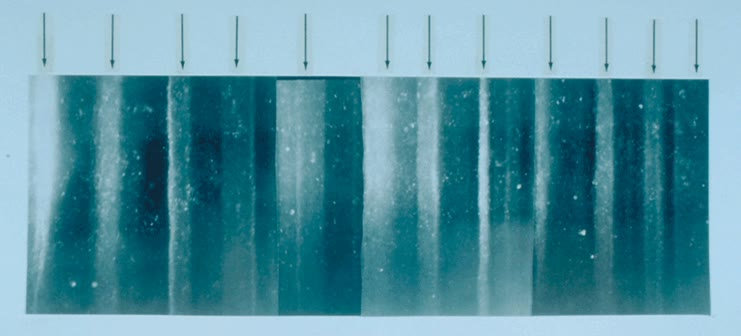
\includegraphics[width=0.72\linewidth]{images/book4/b2-24-gisp2-layers.jpg}
\par\smallskip{\small Un tramo del testigo de hielo GISP2 del centro de Groenlandia, de \qty{1855}{m}
de profundidad, iluminado desde abajo, con capas de verano y de invierno alternadas (las flechas son las de la
diapositiva original). Durante el verano boreal seco, el viento lleva al casquete polvo del Ártico canadiense y de la costa de
Groenlandia.
(Anthony Gow, U.S.\ Army Corps of Engineers CRREL, NOAA Paleoclimatology slide set, dominio público,
a través de Wikimedia Commons.)}
\end{omfigure}
% ledger: photo:b2-24-gisp2, noaa:gisp2-layers

\begin{inthelab}[Cortar un testigo de hielo]
\begin{minipage}[t]{0.54\linewidth}\vspace{0pt}
En una instalación nacional de testigos de hielo, los testigos se guardan en tubos, un metro de testigo por tubo, en un
congelador de archivo a \qty{-36}{\celsius}; los científicos trabajan en una sala de examen a
\qty{-24}{\celsius}. Cuando llega un testigo nuevo, se organiza una línea de procesado: científicos y
técnicos miden, catalogan y cortan cada tramo, típicamente de 30 a \qty{35}{m} al día, de modo que un
testigo de \qty{1000}{m} de longitud lleva de seis a ocho semanas. Un investigador alisa el testigo con un
cepillo y mide su conductividad eléctrica, una clave para definir y datar las capas; otro
sierra los trozos cuyo aire atrapado se analizará para medir el dióxido de carbono y el metano; las muestras se
envían después a los laboratorios que las miden. En EPICA Dome C, cada muestra del perfil de $\delta$D
era de \qty{55}{cm} de hielo.
\end{minipage}\hfill
\begin{minipage}[t]{0.42\linewidth}\vspace{0pt}
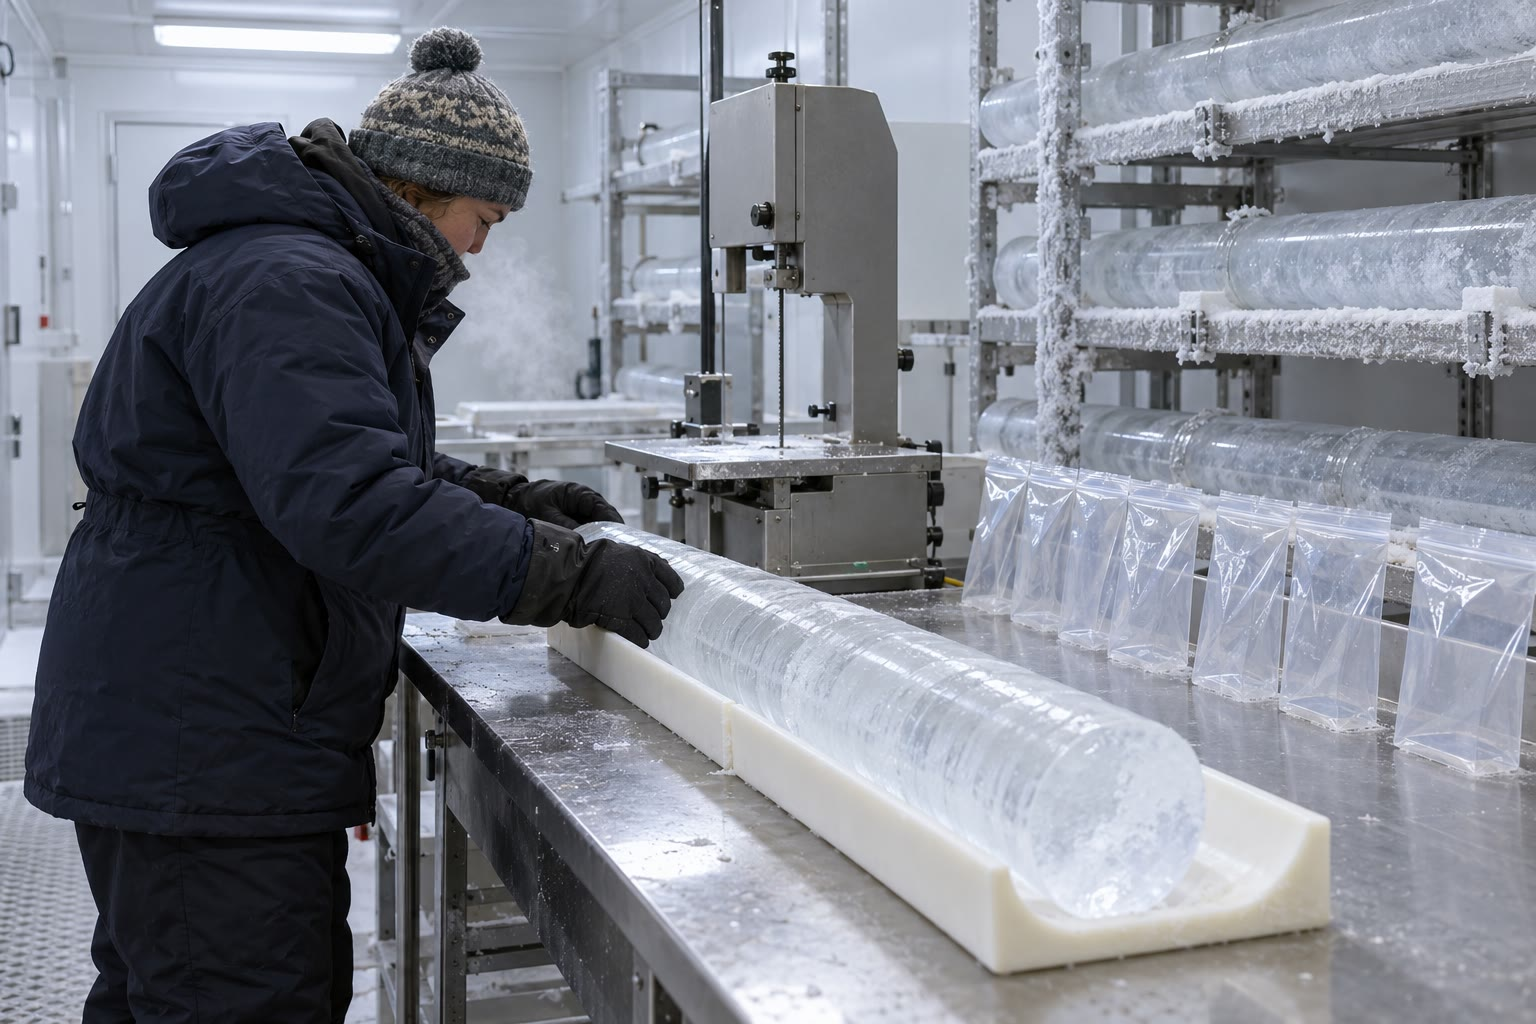
\includegraphics[width=\linewidth]{images/book4/ai/b2-24-cold-lab.jpg}

{\scriptsize Un tramo de testigo de hielo sobre la mesa de un laboratorio frío, junto a una sierra de cinta y bolsas
de muestras (ilustración generada por IA).}
\end{minipage}
\end{inthelab}
% ledger: nsficf:cpl, jouzel07:edc-corr

\section{Otros indicadores, otros archivos}\label{sec:b2:climate-proxies:others}

\subsection*{El magnesio de los caparazones}

La calcita de los foraminíferos incorpora un poco de magnesio en lugar de calcio, y más cuanto
más cálida es el agua. La razón no depende de la composición isotópica del agua, así que
da la temperatura que necesita la ecuación del $\delta^{18}$O.

\begin{definition}[Razón Mg/Ca (indicador)]\label{def:b2:climate-proxies:mgca}
La \emph{razón Mg/Ca (indicador)}\index{razon Mg/Ca (indicador)@razón Mg/Ca (indicador)} es la razón entre magnesio y calcio en
la calcita de los caparazones de foraminíferos, en \unit{mmol/mol}, usada como medida de la temperatura del
agua en la que creció el caparazón mediante una calibración exponencial
\[
  \text{Mg/Ca} = B\,\mathrm{e}^{A T},
\]
con $A$ próximo a \qty{0.09}{\per\celsius} para las especies planctónicas y $B$ propio de cada especie.
\end{definition}
% ledger: groeneveld19:anand, morley24:mgca, miller20:paleotemp

Con $A = 0.09$ la razón crece un $\mathrm{e}^{0.09} - 1 = \qty{9.4}{\percent}$ por grado,
cualquiera que sea la temperatura. Para una especie planctónica de aguas frías, la calibración predicha a partir de
la temperatura sola es $\text{Mg/Ca} = 0.4\,\mathrm{e}^{0.09T}$; un ajuste a 235 caparazones de pescas de
plancton y de techos de testigos del Atlántico Norte da $0.372\,\mathrm{e}^{0.0936T}$, con $r^2 = 0.90$.
A bajas temperaturas las razones medidas se apartan de la curva, y la desviación se atribuye a
la concentración de ion carbonato en el agua de mar: un indicador rara vez depende de una sola variable.
Las especies bentónicas son menos sensibles, unos \qty{0.1}{mmol/mol} por grado para las especies pobres en magnesio
que viven en el sedimento.
% ledger: morley24:mgca, wharton26:deep

\begin{omfigure}
\centering
% figdata/bachelor-2/proxies.py part calib
\begin{tikzpicture}
\begin{groupplot}[group style={group size=2 by 1, horizontal sep=1.7cm},
  tick label style={font=\scriptsize}, label style={font=\small}, height=5.2cm,
  width=0.48\linewidth]
\nextgroupplot[xmin=-2, xmax=14, ymin=0, ymax=3.8, xlabel={$T$ (\unit{\celsius})},
  ylabel={$\delta^{18}\mathrm{O}_{\mathrm{b}} - \delta^{18}\mathrm{O}_{\mathrm{sw}}$ (por mil)},
  xtick={0,4,...,12}, title={a\enspace $\delta^{18}$O bentónico}, title style={font=\scriptsize}]
\addplot[black, thick] table[x=T, y=dd_benthic] {figdata/out/bachelor-2-proxies-calib.dat};
\nextgroupplot[xmin=0, xmax=30, ymin=0, ymax=6.5, xlabel={$T$ (\unit{\celsius})},
  ylabel={Mg/Ca (\unit{mmol/mol})}, xtick={0,5,...,30}, title={b\enspace Mg/Ca planctónico},
  title style={font=\scriptsize},
  legend style={font=\scriptsize, at={(0.03,0.97)}, anchor=north west, draw=none},
  legend cell align=left]
\addplot[ocRed, thick] table[x=T, y=mgca_pred] {figdata/out/bachelor-2-proxies-calib.dat};
\addlegendentry{$0.4\,\mathrm{e}^{0.09T}$}
\addplot[ocBlue, thick, densely dashed] table[x=T, y=mgca_fit]
  {figdata/out/bachelor-2-proxies-calib.dat};
\addlegendentry{$0.372\,\mathrm{e}^{0.0936T}$}
\end{groupplot}
\end{tikzpicture}
\par\smallskip{\small Dos calibraciones. (a) La calibración bentónica de la
\cref{prop:b2:climate-proxies:benthic}: la calcita es más pesada que el agua (cada una en su
escala) en \num{0.21} por mil más por cada grado de enfriamiento. (b) La razón Mg/Ca de una especie
planctónica, predicha a partir de la temperatura sola y ajustada a 235 caparazones.}
\end{omfigure}
% ledger: miller20:paleotemp, morley24:mgca

Medidos en los mismos caparazones, Mg/Ca y $\delta^{18}$O dan dos ecuaciones para dos incógnitas: Mg/Ca
da $T$, y la \cref{prop:b2:climate-proxies:benthic} da entonces
$\delta^{18}\mathrm{O}_{\mathrm{sw}}$, la señal del volumen de hielo. Aplicado a caparazones bentónicos del
Atlántico noroccidental profundo, el método encuentra el agua del Último Máximo Glacial solo unos
\qty{2}{\celsius} más fría que la actual ($-1.78 \pm \qty{0.56}{\celsius}$), mientras que las estimaciones a partir de
las aguas intersticiales sitúan las dos masas de agua profunda cerca de la congelación en el océano glaciar, $-1.1$ y
\qty{-1.9}{\celsius}, donde hoy están entre 2 y \qty{4}{\celsius} y entre 0 y \qty{1}{\celsius}.
% ledger: miller20:paleotemp, wharton26:deep

\subsection*{Los anillos de los árboles}

\begin{definition}[Dendroclimatología; sincronización]\label{def:b2:climate-proxies:dendro}
La \emph{dendroclimatología}\index{dendroclimatologia@dendroclimatología} es la reconstrucción del clima pasado a partir de los
anillos anuales de crecimiento de los árboles: su anchura, la densidad de su madera y su composición
isotópica. La \emph{sincronización}\index{sincronizacion@sincronización} es el emparejamiento de la secuencia de anillos anchos y
estrechos entre árboles, que asigna a cada anillo su año absoluto del calendario y revela
anillos ausentes localmente en un solo árbol.
\end{definition}
% ledger: bebchuk26:crossdating, bebchuk26:absent-rings, ncei:tree-ring, ncei:proxy

Un anillo es más ancho cuando las condiciones favorecen el crecimiento. La \omterm{def:b2:climate-proxies:dendro}{sincronización} es fiable en sitios de clima extremo, donde un
factor climático limita el crecimiento de todos los árboles, de modo que comparten la misma secuencia; puede
fallar donde ningún factor domina, y donde faltan localmente muchos anillos.
Solapar las secuencias de árboles vivos, de maderas antiguas y de madera enterrada alarga una cronología hacia atrás
año a año; un estudio reciente dató una cronología de 100 tejos subfósiles del este de Inglaterra en los
456 años que van de 2668 a 2213 a.\,C., usando el $\delta^{18}$O de más de \num{1500} de sus anillos
frente a una cronología de robles datada de forma absoluta. El International Tree-Ring Data Bank guarda las anchuras de
anillos, densidades, isótopos y cronologías de más de \num{5000} sitios en seis continentes.
% ledger: ncei:proxy, bebchuk26:crossdating, bebchuk26:absent-rings, ncei:tree-ring

\subsection*{Cuevas y lagos}

\begin{definition}[Espeleotema; varva]\label{def:b2:climate-proxies:archives}
Un \emph{espeleotema}\index{espeleotema} es un depósito mineral formado a partir del agua subterránea dentro de una
cueva: estalagmitas, estalactitas y otras formas. Una \emph{varva}\index{varva} es
el depósito de un año en un sedimento lacustre o del fondo marino, normalmente un par de láminas de
composición contrastada, una depositada en verano y otra en el resto del año.
\end{definition}
% ledger: ncei:speleothem, mccarthy23:varves

Los \omterm{def:b2:climate-proxies:archives}{espeleotemas} crecen capa a capa a partir del agua subterránea que llega a una cueva; el espesor de
sus capas y sus registros isotópicos dan las condiciones climáticas pasadas. Algunos tienen bandas anuales,
y algunos contienen compuestos que pueden datarse radiométricamente. La escala de tiempo de los testigos de Groenlandia concuerda con la de
los \omterm{def:b2:climate-proxies:archives}{espeleotemas} de la cueva de Hulu con una diferencia inferior a 800 años en los últimos \num{60000} años: dos
archivos, datados por métodos distintos, se comprueban mutuamente.
% ledger: ncei:speleothem, svensson08:gicc05

\begin{omfigure}
\centering
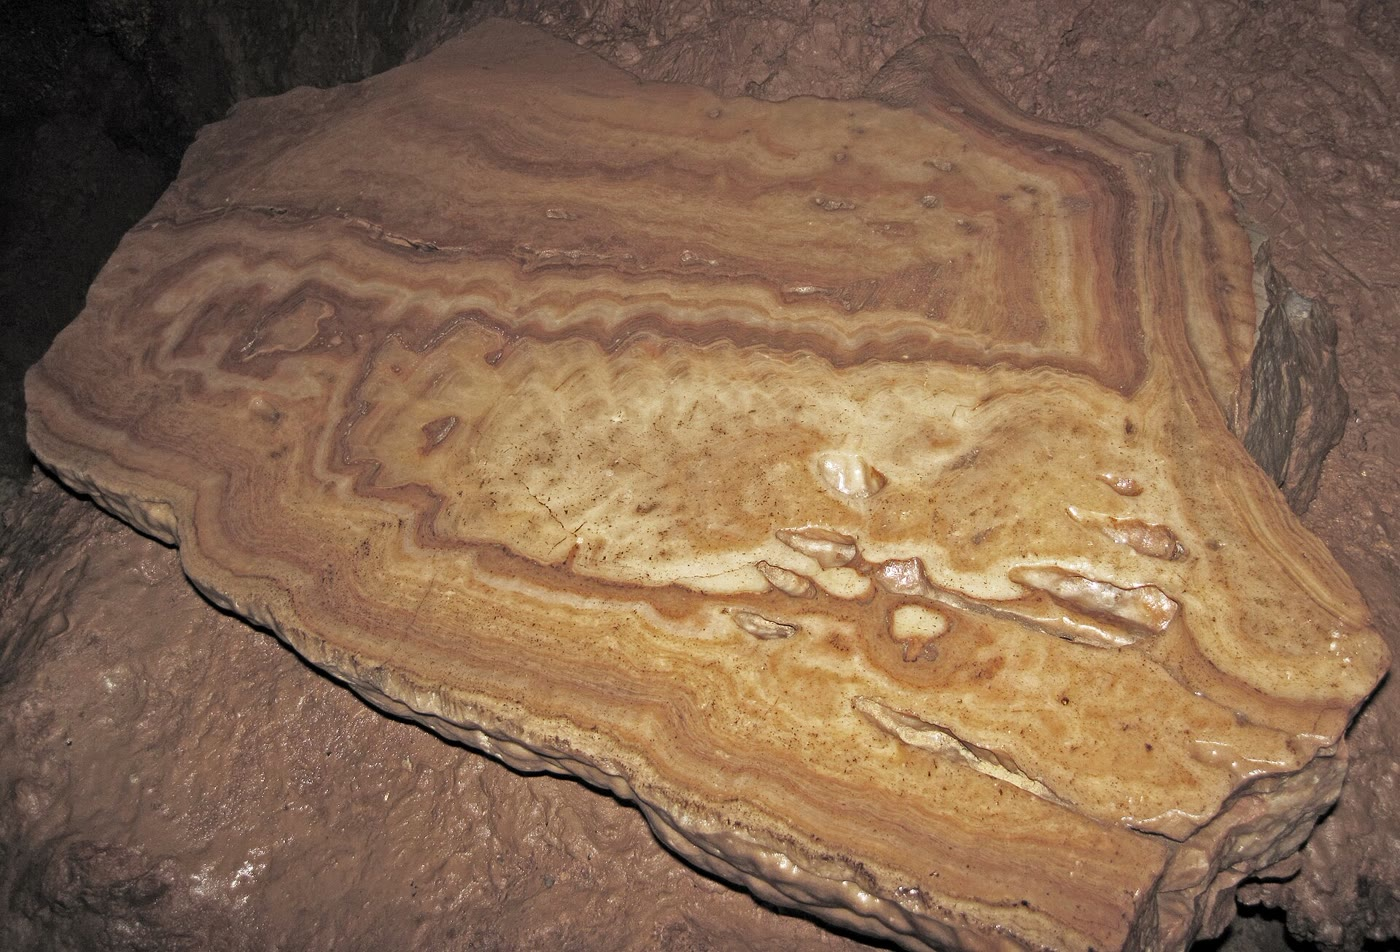
\includegraphics[width=0.62\linewidth]{images/book4/b2-24-speleothem.jpg}
\par\smallskip{\small Una sección cortada y pulida de un \omterm{def:b2:climate-proxies:archives}{espeleotema} de calcita de Diamond Caverns
(Kentucky), coloreada por impurezas de óxido de hierro: cada banda fue en su día la superficie del depósito.
(James St.~John, CC BY 2.0, a través de Wikimedia Commons.)}
\end{omfigure}
% ledger: photo:b2-24-speleothem

En la cubeta profunda del lago Crawford, en Ontario, el agua del fondo, más salada y más alcalina que
el agua de encima, no alberga animales lo bastante grandes para remover el fango, aunque está bien
oxigenada, y cada año añade un doblete: una capa de materia orgánica, cubierta por la
calcita que precipita cada verano a partir del agua superficial alcalina. Los sedimentos lacustres también conservan
el polen de la vegetación circundante, que lee el análisis polínico; con \omterm{def:b2:climate-proxies:archives}{varvas} o sin ellas, registran
la tierra.
% ledger: mccarthy23:varves, mccarthy23:no-bioturbation, ncei:pollen

\section{Los modelos de edad}\label{sec:b2:climate-proxies:age}

Un indicador sin fecha es una curiosidad. Todo archivo necesita una relación entre la profundidad, o el anillo, o la
banda, y la edad.

\begin{definition}[Modelo de edad; recuento de capas anuales]\label{def:b2:climate-proxies:age-model}
Un \emph{modelo de edad}\index{modelo de edad} es la función que asigna una edad, con su incertidumbre, a
cada profundidad de un archivo. El \emph{recuento de capas anuales}\index{recuento de capas anuales} construye un modelo
de edad contando, de arriba abajo, las capas que registran cada una un año (capas de hielo, \omterm{def:b2:climate-proxies:archives}{varvas},
bandas), y cada capa de naturaleza anual dudosa se cuenta como medio año más o menos
medio año.
\end{definition}
% ledger: svensson08:gicc05, mccarthy23:varves

\begin{method}[Construir un modelo de edad]\label{met:b2:climate-proxies:age-model}
\begin{enumerate}
  \item Donde el archivo tiene capas anuales, cuéntense a partir de un techo conocido, anotando aparte las
        dudosas.
  \item Donde no las tiene, o no pueden resolverse, fíjense \emph{puntos de anclaje}: profundidades datadas
        de forma independiente, por radiocarbono u otros métodos radiométricos, por una ceniza volcánica datada, o por
        correlación con un registro bien datado.
  \item Entre los puntos de anclaje, interpólese, linealmente en profundidad si no se sabe nada mejor, o con un
        modelo de cómo se acumuló y adelgazó el archivo.
  \item Propáguese la incertidumbre de cada paso a cada profundidad.
\end{enumerate}
\end{method}
% ledger: svensson08:gicc05, noaa:gisp2-layers, ncei:speleothem

La Greenland Ice Core Chronology 2005, GICC05, cuenta capas anuales en tres testigos de Groenlandia, y
en la parte glaciar solo en el testigo NorthGRIP, a lo largo de los últimos \num{60000} años; sus edades se
dan en años antes del 2000 d.\,C., escritas b2k. Las capas dudosas, contadas como $\frac12 \pm \frac12$,
suman el \emph{error máximo de recuento}, que los autores consideran equivalente a dos desviaciones típicas.
Al comienzo del Holoceno, hace 11\,703 años b2k, es de 50 años; al comienzo del
interestadial de Groenlandia 17, \num{59440} años b2k, es de \num{1287} años.
% ledger: svensson08:gicc05, svensson08:table1

\begin{proposition}[Crecimiento de un error de recuento]\label{prop:b2:climate-proxies:counting}
Sea un recuento que contiene $n$ capas dudosas, cada una contada como $\frac12$ con un error de desviación
típica $\frac12$. Si los errores de las capas son independientes, la desviación típica del
total es $\frac12\sqrt{n}$; si son todos del mismo signo, el error del total es
$\frac12 n$.
\end{proposition}

\begin{proof}
La varianza de una suma de errores independientes es la suma de sus varianzas: $n \times
(\frac12)^2$, cuya raíz cuadrada es $\frac12\sqrt{n}$. Si todas las capas se equivocan en el mismo sentido, los
errores se suman como números: $n \times \frac12$.
\end{proof}

En GI-17, los \num{1287} años de error máximo de recuento suponen \num{2574} capas dudosas. Si
sus errores fueran independientes, el total solo sería incierto en $\frac12\sqrt{2574} = 25$ años.
La suma lineal es la opción prudente: las capas dudosas de un tramo de hielo las juzgan
los mismos contadores con los mismos criterios, y no hay razón para esperar que sus errores se compensen.
La parte más antigua del registro la contaron de forma independiente dos de los autores; sus recuentos
difieren en menos que el error absoluto, aunque localmente en más que el error de recuento final. El
error máximo de recuento promedia aproximadamente un \qty{1}{\percent} del tiempo que abarca un tramo en el Holoceno y un
\qty{5}{\percent} en la parte glaciar.
% ledger: svensson08:gicc05, svensson08:table1, svensson08:two-counters

\begin{omfigure}
\centering
% figdata/bachelor-2/proxies.py part gicc05
\begin{tikzpicture}
\begin{groupplot}[group style={group size=2 by 1, horizontal sep=1.7cm},
  tick label style={font=\scriptsize}, label style={font=\small}, height=5.4cm,
  width=0.48\linewidth, xmin=0, xmax=62, xlabel={edad GICC05 (\unit{ka} b2k)}]
\nextgroupplot[ymin=1450, ymax=2450, y dir=reverse, ylabel={profundidad en NorthGRIP (\unit{m})},
  title={a\enspace profundidad y edad}, title style={font=\scriptsize}]
\addplot[black, mark=*, mark size=1.1pt] table[x=age_ka, y=depth_m]
  {figdata/out/bachelor-2-proxies-gicc05.dat};
\nextgroupplot[ymode=log, ymin=2, ymax=30000, ylabel={incertidumbre (años)},
  title={b\enspace incertidumbre del recuento}, title style={font=\scriptsize},
  legend style={font=\scriptsize, at={(0.03,0.97)}, anchor=north west, draw=none},
  legend cell align=left]
\addplot[ocRed, mark=*, mark size=1.1pt] table[x=age_ka, y=err_yr]
  {figdata/out/bachelor-2-proxies-gicc05.dat};
\addlegendentry{error máximo de recuento}
\addplot[ocBlue, mark=o, mark size=1.1pt] table[x=age_ka, y=err_random_yr]
  {figdata/out/bachelor-2-proxies-gicc05.dat};
\addlegendentry{si fueran independientes}
\end{groupplot}
\end{tikzpicture}
\par\smallskip{\small La cronología GICC05 en 18 eventos climáticos, desde el comienzo del Holoceno hasta
\qty{59.44}{ka}: (a) profundidad en el testigo NorthGRIP frente a la edad; la curva se aplana a medida que las capas
anuales se adelgazan con la profundidad, y cada milenio ocupa menos metros de hielo; (b) el error máximo de recuento, y el error que daría el mismo número de capas
dudosas si sus errores fueran independientes (\cref{prop:b2:climate-proxies:counting});
escala logarítmica. Datos: Svensson et al.\ (2008), tabla 1.}
\end{omfigure}
% ledger: svensson08:table1, svensson08:gicc05

Las capas anuales se adelgazan con la profundidad, porque el hielo fluye y se extiende al hundirse: entre el comienzo
del Holoceno y GI-1, la capa media mide \qty{3.75}{cm} de espesor en NorthGRIP; entre GI-16 y
GI-17, \qty{1.54}{cm}; hacia los \qty{100}{ka}, los modelos de flujo la sitúan cerca de \qty{1}{cm}. Cuanto más delgadas las capas, más difícil
es distinguirlas.
% ledger: svensson08:table1, svensson08:gicc05

\section{La calibración}\label{sec:b2:climate-proxies:calibration}

Toda cifra leída en un indicador pasa por una calibración.

\begin{definition}[Calibración de un indicador]\label{def:b2:climate-proxies:calibration}
La \emph{calibración de un indicador}\index{calibracion de un indicador@calibración de un indicador} es la relación empírica o teórica que
convierte el valor de un indicador en la variable climática que representa, establecida sobre muestras para
las que se conocen ambos, junto con su incertidumbre y el intervalo de condiciones en el que es
válida.
\end{definition}
% ledger: morley24:mgca, miller20:paleotemp

Las muestras para las que se conocen ambos son modernas: caparazones capturados en pescas de plancton, techos de testigos de sedimento comparados con el agua que tienen encima, nieve reciente comparada con la
temperatura de su sitio, los anillos exteriores de los árboles comparados con los registros de una estación meteorológica.
La relación se ajusta después por mínimos cuadrados; para una ley exponencial como la calibración Mg/Ca
el ajuste se hace sobre el logaritmo, que convierte $\text{Mg/Ca} = B\,\mathrm{e}^{AT}$ en
la recta $\ln(\text{Mg/Ca}) = \ln B + AT$. Una calibración se valida con muestras que
no se usaron para ajustarla: se aparta una parte de los datos modernos y se predice.
% ledger: morley24:mgca, werner18:slopes, ncei:tree-ring

Quedan tres límites. Una calibración medida en el espacio, de un lugar a otro en la actualidad, puede no valer
en el tiempo, como ha mostrado el hielo de Groenlandia. Una calibración medida en el intervalo actual de condiciones
debe extrapolarse con cuidado: la razón Mg/Ca de los caparazones se aparta de su ley a bajas temperaturas, donde
otra variable, el ion carbonato, toma el relevo. Y una relación lineal en un intervalo pequeño
puede no serlo en uno grande, como no lo es el \omterm{def:b2:climate-proxies:ice-volume}{efecto del volumen de hielo}. El método de este capítulo
responde a todos ellos de la misma manera: medir dos indicadores independientes en la misma muestra, y que cada uno
compruebe al otro.
% ledger: werner18:slopes, morley24:mgca, rohling21:linear

\section*{Ejercicios}\label{sec:b2:climate-proxies:exercises}

Datos de los ejercicios, salvo aviso contrario: profundidad media del océano $H = \qty{3682.2}{m}$, área del
océano \qty{361.84e6}{km^2}; la calibración bentónica de la \cref{prop:b2:climate-proxies:benthic}; la
calibración planctónica $\text{Mg/Ca} = 0.4\,\mathrm{e}^{0.09T}$ (\unit{mmol/mol}, \unit{\celsius});
valores $\delta$ de las aguas y del hielo en por mil \omterm{def:b2:isotope-geochemistry:standards}{VSMOW}, de la calcita en por mil \omterm{def:b2:isotope-geochemistry:standards}{VPDB}.
% ledger: charette:ocean-volume, miller20:paleotemp, morley24:mgca

\begin{exercise}[$\star$]\label{exo:b2:climate-proxies:1}
Hoy el hielo continental contiene unos \qty{27.5e6}{km^3} y el océano \qty{1350e6}{km^3} de
agua (tómense los volúmenes como cantidades de agua). (a) Si el hielo tiene un $\delta^{18}$O medio de $-30$ por
mil y el océano 0, ¿cuál es el $\delta^{18}$O de toda la hidrosfera, despreciando el agua
dulce? (b) Si se fundiera todo el hielo, ¿en qué se convertiría el $\delta^{18}$O del océano? (c) ¿Qué
fracción del agua es hielo?
\end{exercise}
% ledger: white13c9:ice-mass

\begin{exercise}[$\star$]\label{exo:b2:climate-proxies:2}
Un caparazón bentónico tiene $\delta^{18}\mathrm{O}_{\mathrm{b}} = 2.50$ por mil. (a) Calcúlese su
temperatura si el agua de mar tenía $\delta^{18}\mathrm{O}_{\mathrm{sw}} = 0$. (b) Calcúlese si el
agua de mar tenía $+1.0$ por mil. (c) Otro caparazón, de la misma agua a $0$ por mil, tiene
$2.71$ por mil: ¿cuánto más fría era su agua?
\end{exercise}
% ledger: miller20:paleotemp

\begin{exercise}[$\star$]\label{exo:b2:climate-proxies:3}
(a) Calcúlese la razón Mg/Ca de la calibración planctónica a \qty{10}{\celsius} y a
\qty{20}{\celsius}. (b) ¿En qué factor crece la razón en esos diez grados, y en qué
porcentaje por grado? (c) Calcúlese la temperatura de caparazones con Mg/Ca = 2.0 y
\qty{1.0}{mmol/mol}.
\end{exercise}
% ledger: morley24:mgca

\begin{exercise}[$\star$]\label{exo:b2:climate-proxies:4}
Una cronología de tejos subfósiles va de 2668 a 2213 a.\,C. (a) ¿Cuántos años abarca,
contando ambos años extremos? (b) ¿Por qué una cronología construida con muchos árboles merece más confianza que
el recuento de los anillos de un solo árbol? (c) ¿Por qué cabría esperar que la \omterm{def:b2:climate-proxies:dendro}{sincronización} fuera más fácil para
árboles cercanos al límite frío del bosque que para árboles de un bosque de llanura templado y húmedo?
\end{exercise}
% ledger: bebchuk26:crossdating

\begin{exercise}[$\star\star$]\label{exo:b2:climate-proxies:5}
(a) Con la \cref{prop:b2:climate-proxies:mass-balance}, calcúlese el \omterm{def:b2:climate-proxies:ice-volume}{efecto del volumen de hielo} para un descenso
del nivel del mar de \qty{125}{m} y de \qty{134}{m}, con hielo a $-40$ por mil. (b) Calcúlese para
\qty{130}{m} con hielo a $-30$, $-35$ y $-50$ por mil. (c) ¿Qué composición media del hielo
haría que el efecto de un descenso de \qty{130}{m} igualara los \num{1.0} por mil medidos en las aguas
intersticiales? Compárese con las composiciones de los casquetes actuales.
\end{exercise}
% ledger: ipcc:lgm-sea, white:d18o, miller20:ice-cal, wharton26:deep

\begin{exercise}[$\star\star$]\label{exo:b2:climate-proxies:6}
Compárense las dos calibraciones de la razón Mg/Ca de una misma especie planctónica: la predicha a partir de la
temperatura sola, $0.4\,\mathrm{e}^{0.09T}$, y el ajuste $0.372\,\mathrm{e}^{0.0936T}$. (a) ¿A
qué temperatura coinciden? (b) A \qty{2}{\celsius}, ¿en qué porcentaje es la razón ajustada
menor que la predicha? (c) Un caparazón que creció a \qty{2}{\celsius} sigue la ley ajustada; ¿qué
temperatura le daría la ley predicha?
\end{exercise}
% ledger: morley24:mgca

\begin{exercise}[$\star\star$]\label{exo:b2:climate-proxies:7}
En el testigo NorthGRIP, el comienzo del Holoceno está a \qty{1492.45}{m} y \num{11703} años
b2k, el comienzo de GI-1 a \qty{1604.64}{m} y \num{14692} años; el comienzo de GI-16 a
\qty{2402.55}{m} y \num{58280} años, y el de GI-17 a \qty{2420.44}{m} y \num{59440} años.
(a) Calcúlese el espesor medio de las capas anuales en cada intervalo. (b) ¿Por qué son más delgadas
a mayor profundidad? (c) ¿Por qué el \omterm{def:b2:climate-proxies:age-model}{recuento de capas anuales} se vuelve imposible a cierta profundidad?
\end{exercise}
% ledger: svensson08:table1, svensson08:gicc05

\begin{exercise}[$\star\star$]\label{exo:b2:climate-proxies:8}
Úsense los dos primeros puntos de anclaje del \cref{exo:b2:climate-proxies:7}, con errores máximos de recuento de 50
y 93 años. (a) Por interpolación lineal en profundidad, dese la edad del hielo a \qty{1550}{m}.
(b) Exprésese en años antes de 1950. (c) Interpólese la incertidumbre del mismo modo.
\end{exercise}
% ledger: svensson08:table1

\begin{exercise}[$\star\star$]\label{exo:b2:climate-proxies:9}
El error máximo de recuento de GICC05 es de 93 años en GI-1 y de \num{1287} años en GI-17. (a) ¿Cuántas
capas dudosas representa cada uno? (b) ¿Cuál sería la incertidumbre si los errores de esas
capas fueran independientes, cada uno de desviación típica medio año? (c) ¿En qué factor supera la
suma lineal a la estimación independiente en cada caso, y por qué crece el factor con la profundidad?
\end{exercise}
% ledger: svensson08:gicc05, svensson08:table1

\begin{exercise}[$\star\star\star$]\label{exo:b2:climate-proxies:10}
En EPICA Dome C el $\delta$D medio del hielo es de $-396.6$ por mil en los dos últimos milenios
y de $-441.7$ por mil entre 19 y \qty{23}{ka}. (a) La pendiente espacial antártica del $\delta^{18}$O es de
\num{0.8} por mil por grado. Con la \omterm{prop:b2:isotope-geochemistry:mwl}{recta de agua meteórica}, conviértase en una pendiente de $\delta$D y
estímese el enfriamiento glaciar. (b) El océano glaciar era \num{1.0} por mil más pesado en
$\delta^{18}$O, así que la nieve formada a partir de él también lo era. Suponiendo que el $\delta$D del océano
cambió ocho veces más, corríjase el $\delta$D glaciar y estímese de nuevo el enfriamiento.
(c) La anomalía publicada es de $-0.09$ y \qty{-9.39}{\celsius} para los dos periodos; ¿qué pendiente de
$\delta$D por grado implica, y qué otra corrección contiene la serie publicada?
\end{exercise}
% ledger: data:b4-proxies, werner18:slopes, kc98:mwl, wharton26:deep, jouzel07:edc-corr

\begin{exercise}[$\star\star\star$]\label{exo:b2:climate-proxies:11}
Una calibración de la razón Mg/Ca de una especie planctónica usa seis muestras de techo de testigo (temperatura del agua,
Mg/Ca en \unit{mmol/mol}): (4, 0.59), (8, 0.80), (12, 1.21), (16, 1.65), (20, 2.47), (24, 3.41).
(a) Ajústese $\ln(\text{Mg/Ca}) = \ln B + AT$ por mínimos cuadrados, y dense $A$ y $B$. (b) Calcúlense los
residuos del logaritmo, y compárese el ajuste con la ley $0.4\,\mathrm{e}^{0.09T}$. (c) Dese la
temperatura de un caparazón glaciar con Mg/Ca = 1.30. (d) Un caparazón tiene Mg/Ca = 0.45: calcúlese su
temperatura, y dígase por qué este valor merece menos confianza que el anterior.
\end{exercise}
% ledger: morley24:mgca

\begin{exercise}[$\star\star\star$]\label{exo:b2:climate-proxies:12}
Un casquete de hielo crece en dos etapas: primero se almacenan \qty{60}{m} de nivel del mar como hielo a $-30$ por mil,
después \qty{70}{m} más como hielo a $-45$ por mil. (a) Demuéstrese que el balance de masas de la
\cref{prop:b2:climate-proxies:mass-balance} se convierte en $(H - h)\,\Delta\delta = -\sum_i h_i\delta_i$
para varios depósitos de hielo, y calcúlese el \omterm{def:b2:climate-proxies:ice-volume}{efecto del volumen de hielo} tras cada etapa. (b) ¿Cuál es la composición
media del hielo al final? (c) Una regla lineal, calibrada con el estado final, convierte
$\Delta\delta$ en nivel del mar. ¿Qué descenso del nivel del mar inferiría para la primera etapa, y por qué
se equivoca?
\end{exercise}
% ledger: rohling21:linear, white:d18o, miller20:ice-cal

\begin{problem}[{Problema de fin de semana --- Un caparazón, dos señales}]\label{pb:b2:climate-proxies:1}
¿Cuánto más frío estaba el océano profundo en el Último Máximo Glacial? El $\delta^{18}$O de los caparazones bentónicos
mezcla la respuesta con el volumen del hielo; este problema separa ambos. Úsense los datos de los
ejercicios; el nivel del mar estaba de 125 a \qty{134}{m} por debajo del actual, y se cree que el hielo del casquete de
América del Norte tenía un $\delta^{18}$O de unos $-40$ por mil.

\medskip\noindent\textbf{Parte I --- El hielo en tierra.}
\begin{enumerate}
  \item Calcúlese el volumen de agua retirado del océano por un descenso del nivel del mar de \qty{130}{m}.
  \item Calcúlese el \omterm{def:b2:climate-proxies:ice-volume}{efecto del volumen de hielo} de ese descenso con hielo a $-40$ por mil.
  \item Calcúlese para descensos de \qty{125}{m} y \qty{134}{m}.
  \item Calcúlese para \qty{130}{m} con hielo a $-35$ y a $-50$ por mil. ¿Qué incertidumbre
        importa más, la del nivel del mar o la del hielo?
  \item Las aguas intersticiales de los sedimentos glaciares dan $1.0 \pm 0.1$ por mil. ¿Qué composición media
        del hielo requeriría un descenso de \qty{130}{m} para producirlo?
  \item Calcúlese el desplazamiento por metro de nivel del mar para descensos pequeños con hielo a $-40$ por mil, y
        compárese con el valor de \num{0.011} por mil por metro deducido de niveles del mar datados.
\end{enumerate}

\medskip\noindent\textbf{Parte II --- Dos termómetros.}
\begin{enumerate}[resume]
  \item Demuéstrese a partir de la \cref{prop:b2:climate-proxies:benthic} que un enfriamiento de \qty{1}{\celsius} con
        composición del agua constante aumenta $\delta^{18}\mathrm{O}_{\mathrm{b}}$ en \num{0.21} por mil.
  \item Calcúlese el $\delta^{18}\mathrm{O}_{\mathrm{b}}$ de un caparazón bentónico crecido hoy en agua a
        \qty{2.0}{\celsius} con $\delta^{18}\mathrm{O}_{\mathrm{sw}} = 0$.
  \item Calcúlese para un caparazón glaciar crecido en agua a \qty{-1.0}{\celsius} con
        $\delta^{18}\mathrm{O}_{\mathrm{sw}} = +1.0$ por mil. ¿Cuál es el cambio entre los dos
        caparazones, y qué parte se debe a la composición del agua?
  \item Un caparazón planctónico tiene Mg/Ca = \qty{2.0}{mmol/mol}. Calcúlese su temperatura.
  \item Los caparazones bentónicos pobres en magnesio ganan unos \qty{0.1}{mmol/mol} por grado. Un caparazón glaciar tiene
        una razón Mg/Ca \qty{0.18}{mmol/mol} menor que uno moderno de la misma especie y del mismo
        lugar. ¿Qué enfriamiento indica?
  \item ¿Por qué la razón Mg/Ca da una temperatura que no depende del volumen de hielo?
\end{enumerate}

\medskip\noindent\textbf{Parte III --- El residuo.}
El registro apilado LR04 marca \num{3.23} por mil hoy y \num{4.92} por mil en promedio entre 19 y
\qty{23}{ka}.
\begin{enumerate}[resume]
  \item Calcúlese el cambio del registro apilado entre hoy y el Último Máximo Glacial.
  \item Si todo fuera \omterm{def:b2:climate-proxies:ice-volume}{efecto del volumen de hielo}, con hielo a $-40$ por mil, ¿qué descenso del nivel del mar
        implicaría (inviértase la \cref{prop:b2:climate-proxies:mass-balance})? ¿Es coherente con los
        indicios del nivel del mar?
  \item Tómese el \omterm{def:b2:climate-proxies:ice-volume}{efecto del volumen de hielo} de la pregunta 2. ¿Qué residuo queda para la temperatura, y
        qué enfriamiento del agua profunda da?
  \item Tómese en cambio el valor del agua intersticial, \num{1.0} por mil. ¿Qué residuo y qué enfriamiento?
  \item Otra reconstrucción usa \num{0.25} por mil por grado. Repítanse con ella las dos estimaciones.
  \item Hoy el Agua Profunda del Atlántico Norte está entre 2 y \qty{4}{\celsius} y el Agua Antártica de
        Fondo entre 0 y \qty{1}{\celsius}; las aguas intersticiales las sitúan a $-1.1$ y \qty{-1.9}{\celsius}
        en el océano glaciar, y la razón Mg/Ca de los caparazones bentónicos encuentra el Atlántico noroccidental profundo
        solo unos \qty{1.8}{\celsius} más frío. ¿Qué intervalo de enfriamiento dan, y cuál de las
        dos estimaciones de las preguntas 15 y 16 favorecen?
\end{enumerate}

\medskip\noindent\textbf{Parte IV --- La vista desde el hielo.}
En EPICA Dome C el $\delta$D medio es de $-396.6$ por mil en los dos últimos milenios y de
$-441.7$ por mil entre 19 y \qty{23}{ka}; la anomalía de temperatura publicada es de $-0.09$ y
\qty{-9.39}{\celsius}.
\begin{enumerate}[resume]
  \item Calcúlese el cambio de $\delta$D.
  \item Con una pendiente del $\delta^{18}$O de \num{0.8} por mil por grado y la \omterm{prop:b2:isotope-geochemistry:mwl}{recta de agua meteórica},
        estímese el enfriamiento en Dome C.
  \item Calcúlese el enfriamiento publicado, y la pendiente de $\delta$D por grado que implica.
  \item La superficie media global estaba de 5 a \qty{7}{\celsius} más fría en el Último Máximo Glacial.
        Ordénense los enfriamientos de Dome C, del globo y del océano profundo.
  \item ¿Por qué el océano profundo no puede haberse enfriado tanto como la superficie de la Antártida?
  \item En resumen: con la corrección del volumen de hielo dada por el agua intersticial, ¿cuánto más frío estaba el océano profundo
        en el Último Máximo Glacial que hoy?
\end{enumerate}
\end{problem}
% ledger: charette:ocean-volume, ipcc:lgm-sea, miller20:ice-cal, white:d18o, white13c9:ice-volume, wharton26:deep, miller20:paleotemp, morley24:mgca, data:b4-proxies, rohling21:linear, werner18:slopes, kc98:mwl, ipcc:lgm-cooling
